\section{Preliminaries}

Before understanding the weakest part of the cipher, a clarified concept of cache memory and how they are accessed during real time AES implementation might be helpful.\\

\subsection{Memory Access in AES Implementations}

The memory access patterns of AES are particularly susceptible to cryptanalysis. The cipher is abstractly defined by algebraic operations and could, in principle, be directly implemented using just logical and arithmetic operations. However, performance-oriented software implementations on 32-bit (or higher) processors typically use an alternative formulation based on lookup tables as prescribed in the Rijndael Specification \citep{daemen2002design}.\\

Several lookup tables are precomputed once by the programmer or during system initialization. There are 8 such tables, $T_0,T_1,T_2,T_3$ and $T_0^{10},T_1^{10},T_2^{10},T_3^{10}$, each containing 256 4-byte words. The contents of the tables, defined in \citep{daemen2002design}, are inconsequential to most of the cache-timing attacks because of memory protection.\\

During key setup, a given 16-byte secret key $k=(k_0,k_1,...,k_{15})$ is expanded into 10 round keys, $K^{(r)}$ for $r=1,2,...,10$. Each round is divided into 4 words of 4 bytes each: $K^{(r)}=(K_0^{(r)},K_1^{(r)},K_2^{(r)},K_3^{(r)})$. The 0th round key is just the raw key: $K_j^{(0)}=(k_{4j},k_{4j+1},k_{4j+2},k_{4j+3})$ for $j=0,1,2,3$. The details of the rest of the key expansions are mostly inconsequential \citep{osvik}.\\

Given a 16-byte plaintext $p=(p_0,p_1,...,p_{15})$, encryption proceeds by computing a 16-byte intermediate state $x^{(r)}=(x_0^{(r)},x_1^{(r)},...,x_{15}^{(r)})$ at each round r. The inital state $x^{(0)}$ is computed by $x_i^{(0)}=p_i \oplus k_i ( i=0,1,...,15 )$.

\begin{center}
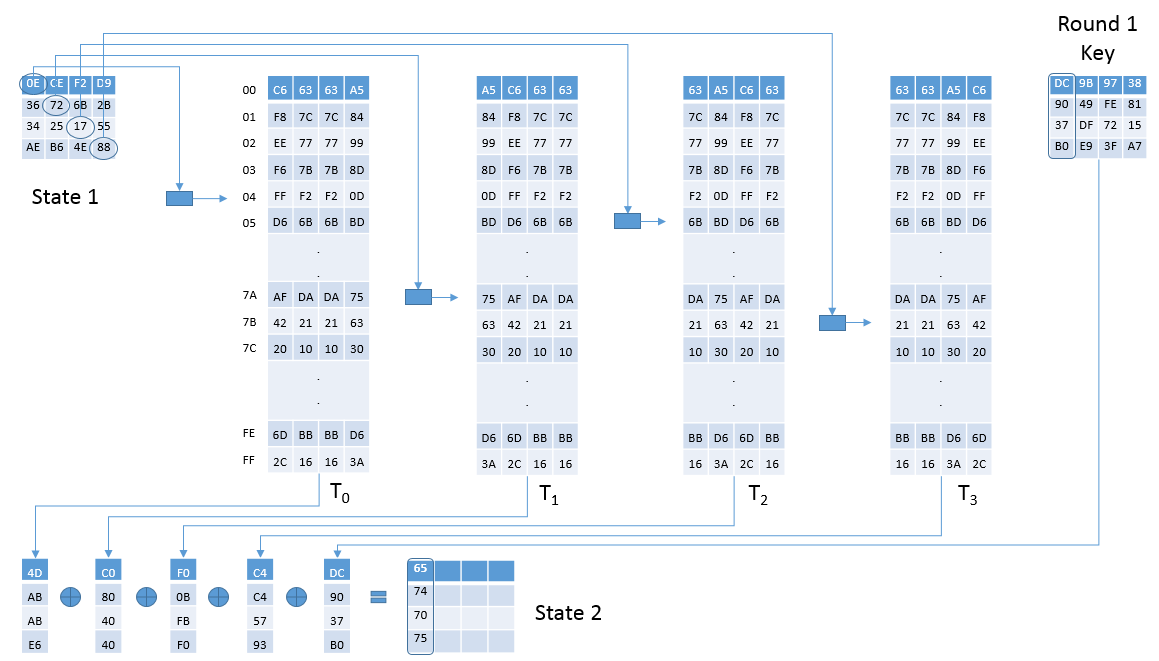
\includegraphics[scale=0.4,natwidth=1159,natheight=661]{Figures/aes-1-1(new).png}
\captionof{figure}{The figure demonstrates how $x_0^1,x_1^1,x_2^1,x_3^1$ are computed. Note that the bytes of the state matrix are being used as index of the lookup tables. Since the lookup table remains the same for a particular S-Box, an index byte will always cause lookup from the same block of cache memory}
\label{fig: The diagram shows how $x_0^1,x_1^1,x_2^1,x_3^1$ are computed.}
\end{center}

\begin{flushleft}
Thus, the first 9 rounds are computed by updating the intermediate state as follows, for $r=0,1,..,8$:
\end{flushleft}
\begin{small}
\begin{align*}
&(x_0^{(r+1)},x_1^{(r+1)},x_2^{(r+1)},x_3^{(r+1)}) \gets T_0[x_0{(r)}] \oplus T_1[x_5{(r)}] \oplus T_2[x_{10}{(r)}] \oplus T_3[x_{15}{(r)}] \oplus K_0^{(r+1)}\\
&(x_4^{(r+1)},x_5^{(r+1)},x_6^{(r+1)},x_7^{(r+1)}) \gets T_0[x_4{(r)}] \oplus T_1[x_9{(r)}] \oplus T_2[x_{14}{(r)}] \oplus T_3[x_{3}{(r)}] \oplus K_0^{(r+1)}\\
&(x_8^{(r+1)},x_9^{(r+1)},x_{10}^{(r+1)},x_{11}^{(r+1)}) \gets T_0[x_8{(r)}] \oplus T_1[x_{13}{(r)}] \oplus T_2[x_{2}{(r)}] \oplus T_3[x_{7}{(r)}] \oplus K_0^{(r+1)}\\
&(x_{12}^{(r+1)},x_{13}^{(r+1)},x_{14}^{(r+1)},x_{15}^{(r+1)}) \gets T_0[x_{12}{(r)}] \oplus T_1[x_1{(r)}] \oplus T_2[x_{6}{(r)}] \oplus T_3[x_{11}{(r)}] \oplus K_0^{(r+1)}
\end{align*}
\end{small}

Finally, to compute the last round, the above process of table-lookup is repeated with $r=9$, except that $T_0,T_1,T_2,T_3$ are replaced by $T_0^{(10)},T_1^{(10)},T_2^{(10)},T_3^{(10)}$. The resulting $x^{(10)}$ is the ciphertext. Compared to the algebraic formulation of AES, here the lookup tables represent the combination of \emph{ShiftRows}, \emph{MixColumns} and \emph{SubBytes} operations; the change of lookup tables in the last round is due to the absence of \emph{MixColumns} \citep{osvik}. It is clear from the above discussion that computation of a state matrix requires 16 Table lookups and 16 XOR operations.\\

We know, the first round state matrix is computed by XOR operation between the 16-byte plain text and the 16 byte plain key. One important point to notice from the previous discussion is that the state bytes are being used as index to the Lookup tables. Thus any Information of the accessed index will directly translate to Encryption Key Byte. For example, lets say we know $x_i^{(0)}$. Since plaintext is known for triggered encryptions, we know $x_i^{(0)}$ too.\\

\begin{align*}
x_i^{(0)} \gets x_i^{(0)} \oplus k_i^{(0)}
\end{align*}


\begin{center}
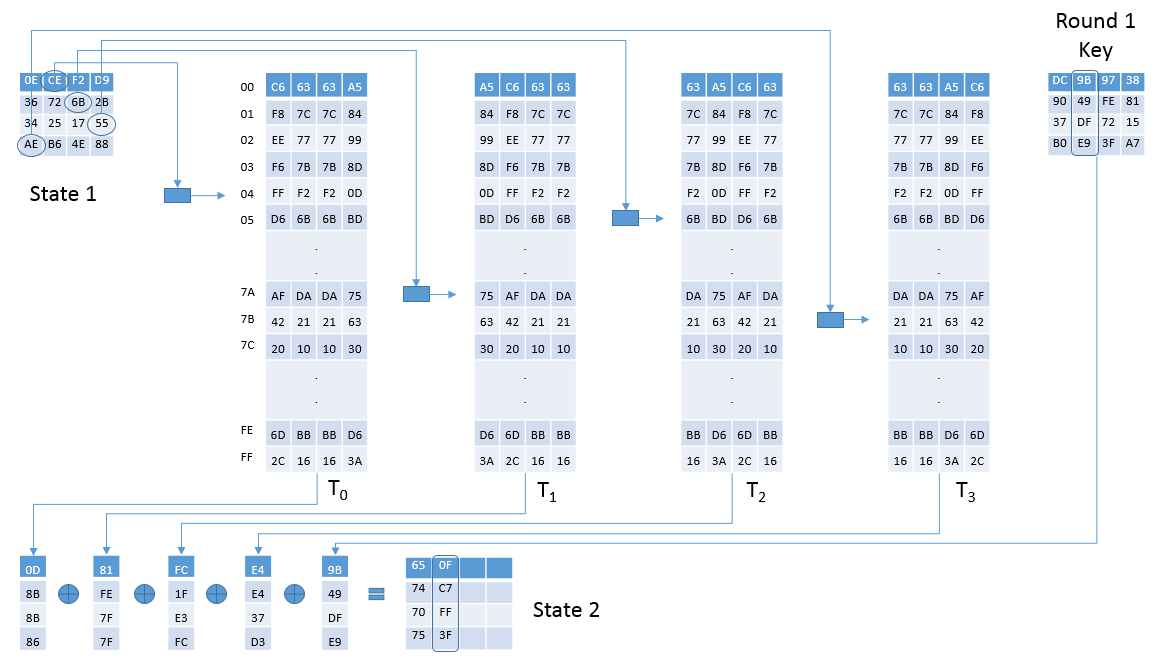
\includegraphics[scale=0.4,natwidth=918,natheight=525]{Figures/aes-1-2(new).png}
\captionof{figure}{The figure demonstrates how $x_4^1,x_5^1,x_6^1,x_7^1$ are computed.}
\label{fig: The diagram shows how $x_4^1,x_5^1,x_6^1,x_7^1$ are computed.}
\end{center}


%\begin{center}
%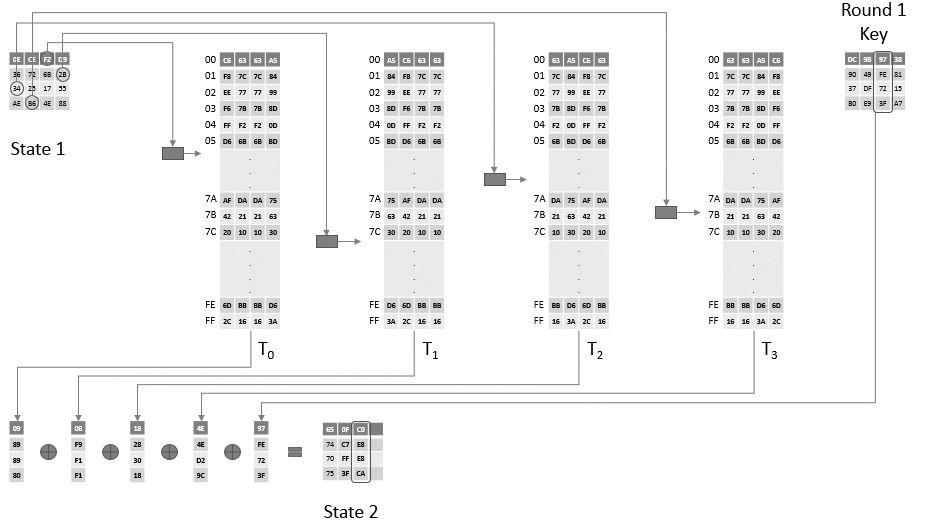
\includegraphics[scale=0.30,natwidth=925,natheight=521]{Figures/aes-1-3.png}
%\captionof{figure}{The diagram shows how $x_8^1,x_9^1,x_{10}^1,x_{11}^1$ are computed}
%\label{fig: The diagram shows how $x_8^1,x_9^1,x_{10}^1,x_{11}^1$ are computed.}

%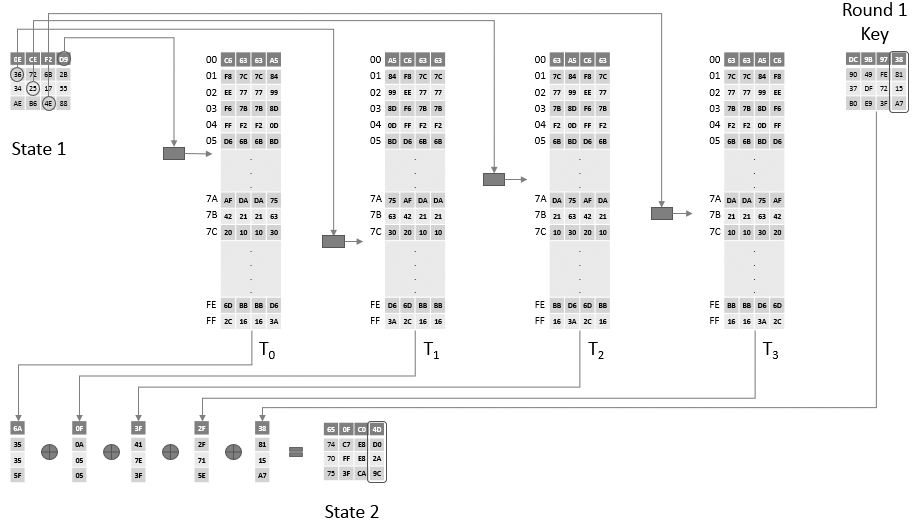
\includegraphics[scale=0.30,natwidth=917,natheight=521]{Figures/aes-1-4.png}
%\captionof{figure}{The diagram shows how $x_{12}^1,x_{13}^1,x_{14}^1,x_{15}^1$ are computed.}
%\label{fig: The diagram shows how $x_{12}^1,x_{13}^1,x_{14}^1,x_{15}^1$ are computed.}
%\end{center}

\begin{flushleft}
This implies,
\end{flushleft}
\begin{align*}
k_i^{(0)} \gets x_i^{(0)} \oplus x_i^{(1)}
\end{align*}

\begin{flushleft}
Thus knowing $x_i^1{(1)}$ for $i=0,1,2,...,15$ is sufficient to recover the full encryption key under the assumption that the plaintext is known. This is the weakest part of Round 1; in fact the weakest part of the Cipher.
\end{flushleft}

\subsection{How Lookup Tables fit in Memory and Cache}

Lets turn our attention to how AES Lookup tables fit in Memory and in Cache. We know, each Lookup table has 256 4-Byte entry. That gives it a total size of $256 \cdot 4=1024$ Bytes. Now, typical size of \emph{memory block} is 64 Bytes even on modern microprocessors. So for simplicity, we will assume the \emph{memory block} size $B$ to be 64 Bytes throughout this paper. Therefore, each table $T_i$ will occupy 16 memory blocks.

\begin{flushleft}
Also assume that, the initial address of $T_i$ congruent to the cache. That is, 1st block of the table will be cached in one of the $W$ \emph{cache lines} in the 1st \emph{cache set}.
\end{flushleft}
